

\section{Methodology}
\subsection{Reward Function}

The training reward of each vehicle is the composite utility $U_{PRR}$ of \Cref{eq:uprr}, evaluated at every decision step and clipped to $[0,1]$ (\Cref{eq:uclip}): $r_t = U_{PRR}(t)$. It combines the empirical packet-reception ratio, a latency term $\exp(-L/D)$ that falls as the completion latency $L$ approaches the task deadline $D$, an energy term $\exp(-E/3)$, and a congestion-change term $\Delta\text{CBR}$, with task-adaptive weights $(\alpha,\beta) = (0.70, 0.30)$ for safety, $(0.40, 0.60)$ for infotainment and $(0.20, 0.80)$ for compute tasks. The deadline-based utility $U_{OTR}$ (\Cref{eq:uotr}) is computed alongside but is used for evaluation only. The energy term carries the limitation disclosed in \Cref{sec:energy_utility}: it is a reward-shaping signal, not a validated energy measure.

\subsection{Deadline Retention Ratio (DRR) Metric}

\subsubsection*{1) Definition and Motivation}

Standard performance metrics (OTR, latency) are evaluated at a single network density (e.g., $N = 32$ vehicles). However, policies trained at one density may degrade rapidly under increasing contention. We introduce the Deadline Retention Ratio ($R_D$, also written $\text{DRR}(N_{\text{test}}, N_{\text{ref}})$) to quantify robustness across fleet sizes.

\begin{equation}
\label{eq:drr_definition}
R_D = \frac{\text{OTR}(N_{\text{test}})}{\text{OTR}(N_{\text{ref}})}
\end{equation}

where $N_{\text{ref}}$ is the reference (smaller) fleet size and $N_{\text{test}}$ is the test (larger) fleet size.

\subsubsection*{2) Computation Algorithm}

\begin{algorithm}
\caption{Deadline Retention Ratio Computation}
\label{alg:drr}
\begin{algorithmic}[1]
\REQUIRE Evaluation logs containing task completion times for both $N_{\text{ref}}$ and $N_{\text{test}}$ scenarios
\ENSURE Scalar $R_D \in [0, 1]$
\STATE $c_{\text{ref}} \gets 0$
\STATE $n_{\text{ref}} \gets 0$
\FOR{each task $\tau$ in reference scenario $(N_{\text{ref}})$}
  \IF{completion\_time$(\tau) \le D_{\max}$}
    \STATE $c_{\text{ref}} \gets c_{\text{ref}} + 1$
  \ENDIF
  \STATE $n_{\text{ref}} \gets n_{\text{ref}} + 1$
\ENDFOR
\STATE $\text{OTR}_{\text{ref}} \gets \frac{c_{\text{ref}}}{n_{\text{ref}}}$
\STATE [Repeat for $N_{\text{test}}$ scenario to compute $\text{OTR}_{\text{test}}$]
\STATE $R_D \gets \frac{\text{OTR}_{\text{test}}}{\text{OTR}_{\text{ref}}}$
\STATE \textbf{return} $R_D$
\end{algorithmic}
\end{algorithm}

\noindent where $c_{\text{ref}}$ is the number of tasks completed within deadline ($D_{\max}$) and $n_{\text{ref}}$ is the total task count in the reference scenario (with $c_{\text{test}}$ and $n_{\text{test}}$ defined analogously).

\subsubsection*{3) Interpretation}
$R_D = 0.94$ means the policy retains 94\% of its reference-density deadline performance when fleet size increases fourfold; $R_D = 0.60$ indicates severe degradation under contention.

\subsection{Federated Learning Hyperparameters}

Table~\ref{tab:hyperparameters} consolidates all D3QN and FedAvg hyperparameters used in training:

\begin{table*}[t]
\caption{Federated D3QN and FedAvg Hyperparameters}
\label{tab:hyperparameters}
\centering
% booktabs-restyled
\footnotesize
\setlength{\tabcolsep}{3pt}
\renewcommand{\arraystretch}{1.15}
\begin{tabularx}{\textwidth}{>{\hsize=1.500\hsize\raggedright\arraybackslash}X>{\hsize=0.600\hsize\centering\arraybackslash}X>{\hsize=0.400\hsize\centering\arraybackslash}X>{\hsize=1.500\hsize\raggedright\arraybackslash}X}
\toprule
\textbf{Parameter} & \textbf{Value} & \textbf{Symbol} & \textbf{Justification} \\
\midrule
\multicolumn{4}{c}{\textbf{Deep Reinforcement Learning (D3QN)}} \\
Learning rate (neural network) & 0.0001 & $\alpha$ & Prevents divergence in double-Q stabilization \\
Discount factor & 0.95 & $\gamma$ & Task completion horizons typically 5--10 seconds \\
Exploration decay ($\epsilon$-greedy) & $0.995^t$ & $\epsilon(t)$ & Linear annealing from 1.0 to 0.05 over training \\
Exploration final rate & 0.05 & $\epsilon_{\min}$ & Preserves exploration throughout training \\
Replay buffer size & 50,000 & $B$ & Trade-off: larger stabilizes, constrained by GPU memory (12 GB) \\
Minibatch size & 64 & batch\_size & Standard for DQN; aligns with GPU optimization \\
Target network update frequency & 1,000 steps & $\tau$ & Reduces temporal correlations \\
Network architecture & $\text{input}-256-256-|A|$ & $\pi$ & Dueling DQN: separate advantage and value streams \\
\midrule
\multicolumn{4}{c}{\textbf{Federated Learning (FedAvg)}} \\
Global aggregation rounds & $K = 5$ & $K$ & Trade-off: communication cost vs. gradient staleness \\
Local training epochs per round & 3 & $E$ & Vehicle trains 3 episodes locally before aggregation \\
Federated learning rate & 0.001 & $\eta_{\text{fed}}$ & Slower than local $\alpha$; ensures stable aggregation \\
Participants (vehicles) & 8, 16, 32 & $N$ & Density-sweep experiments \\
Episodes per participant & 100 & $T$ & Total training = $N \times E \times T$ epochs \\
Gradient clipping threshold & 1.0 & $\text{clip}$ & Prevents exploding gradients in federated setting \\
\bottomrule
\end{tabularx}
\end{table*}


\textbf{Sensitivity notes:} Preliminary ablation studies (not shown for space) validated that $\gamma = 0.95$ and $\alpha_{\text{D3QN}} = 0.0001$ produce convergence. Values of $K \in \{3, 5, 7\}$ showed diminishing returns; $K = 5$ was selected as the mid-point.

\subsection{Simulation Environment Specification}

\subsubsection*{1) Python Framework and Simulator}

The framework is implemented in Python 3.8+ utilizing PyTorch 1.10.0 with CUDA 11.3 for GPU-accelerated deep learning. The MDP simulator is a custom environment class designed without external dependencies on ns-3 or SUMO for the pure-simulation track. Numerical operations are handled by NumPy 1.21.0 and SciPy 1.7.0, while Pandas, Matplotlib, and TensorBoard are used for logging and visualization.

\subsubsection*{2) Vehicle Mobility and Traffic Pattern}

Vehicle mobility follows a Synthetic Random Waypoint model within a $10 \text{ km} \times 10 \text{ km}$ grid. Vehicle speeds are uniformly sampled from 5 to 30 m/s to represent urban to highway conditions, with direction changes occurring every 30 to 60 seconds towards randomly selected waypoints. Task generation is modeled as a Poisson process with an arrival rate of $\lambda = 1$ task per vehicle per second for the URLLC stress scenario, and task sizes follow a log-normal distribution to mimic real V2X compute workloads.

\subsubsection*{3) RAT Parameters and Channel Model}

The per-RAT parameters used by the simulator are those of \Cref{tab:rat_physical}. \textbf{Channel Model:} LTE and 5G-NR links include Jakes (Rayleigh) fading, drawn once per 100 ms step with a loss that depends on the ratio of the step to the coherence time implied by the Doppler frequency (vehicle speed and carrier frequency); ITS-G5 and WiFi-6 use a constant, non-fading channel.

\subsubsection*{4) MEC Server Queue Model}

Each RSU's edge server is modelled as a shared backlog. In every 100 ms step, the backlog $Q_r$ of RSU $r$ is the sum of the offload ratios requested by the vehicles it serves, and each unit of backlog delays every offloading vehicle at that RSU by $\tau = 50$ ms (an effective service rate of 20 tasks/s per RSU). $\tau$ is a modelling constant calibrated for this study. Vehicles observe the backlog normalised by the fleet size, $Q_r/N \in [0,1]$, as a continuous feature.

\subsubsection*{5) Task Completion Time and Deadline Evaluation}

Task completion time follows the end-to-end latency model of \Cref{eq:ltotal_partial}. In the simulator, the queueing delay is $\tau Q_r$ as above, the per-RAT access delay follows \Cref{tab:rat_physical}, remote processing adds 0.5 ms per MB of offloaded data, and local processing runs at 2 GHz. A task $\tau$ is deadline-compliant if its total latency does not exceed its deadline $D_i$.

\subsubsection*{6) Reproducibility Configuration}

To ensure reproducibility, experiments utilize 5 independent random seeds for all training and evaluation runs. Each run comprises 100 training episodes per vehicle per density, with the evaluation window defined as the final 5 episodes post-convergence. The code repository, configuration YAML files, checkpoint weights, and raw evaluation logs are made available in the supplementary materials.


\begin{figure*}[p]
\centering
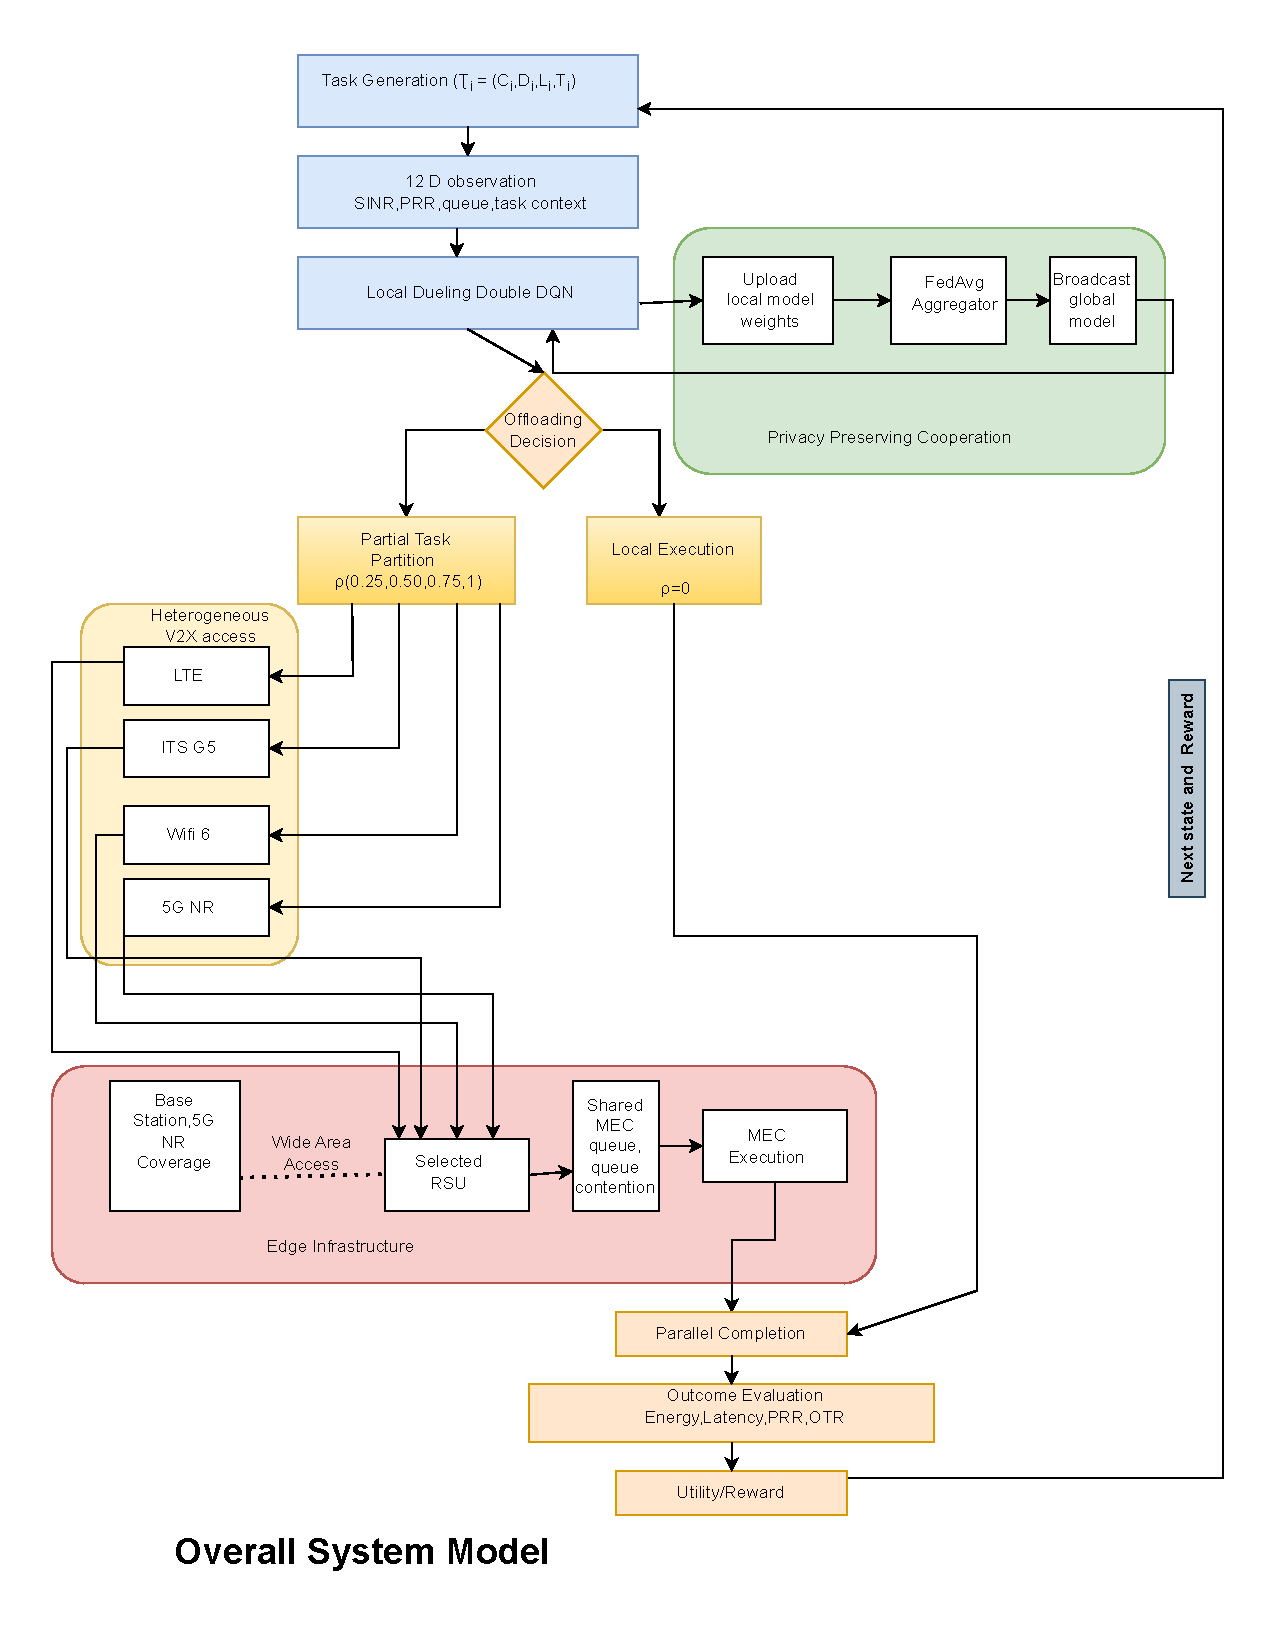
\includegraphics[trim=21bp 62bp 21bp 23bp,clip,height=0.88\textheight,keepaspectratio]{figures/handmade/system_model_a_original.pdf}
\caption{Overall system model showing task offloading flow, MDP state and action space, and end-to-end latency components.}
\label{fig:overall_system_model}
\end{figure*}
